\documentclass{article}
\usepackage{graphicx} % Required for inserting images
\usepackage{biblatex} % For refereces
\usepackage{hyperref}
\addbibresource{bibliography.bib} 
\usepackage[utf8]{inputenc} % 
\usepackage[british]{babel}
\usepackage{xcolor}

\title{\textcolor{blue}{Red} or \textcolor{red}{Blue} Academia?}
\author{\underline{cracked.egg}\\Chloe, Ago, Imar \& Marenthe}
\date{UCACCMET2J\\Winter 2025}

\begin{document}

\maketitle

\section{Introduction}
In recent years, there have been discussions on the presence of political bias in higher education, and generally, universities are said to be left-leaning/liberal. Education plays a significant role in the development of political stances, as they are places where people come into contact with different points of views, during their formative years. To ensure students are able to form their own opinions, one could say that neutrality is essential here. However, full neutrality in education seems difficult to achieve. 

The aim of this study is to investigate whether structural bias exists in higher education institutes, and what its (long-term) impacts on students are. More specifically, do US universities have a bias in the politicians they produce? We will explore whether there is a relationship between the university attended and the political affiliation of politicians in the United States. Furthermore, we are interested in looking for potential explanations for the pattern we might find. As the saying 'money is power' highlights, we think it is worth investigating the impact of the financial status of universities on the political bias within educational institutes. Hence, we will asses how the level on endowments of universities influence the political affiliation of the politicians they bring forth. Lastly, the potential interactions of those different variables will be inspected. 
 
\section{Methods}

The data used was taken from The People of Wikipedia, a dataset containing a large number of Wikipedia pages of people in 2018 \cite{lehmann2015dbpedia}. The People of Wikipedia is part of the DBpedia project, collecting all sorts of data on known people. The relevant variables in the dataset for our study are the person's affiliated political party and the university they attended. The analyses were conducted in Python and R, where the tidyverse package was used for visualizations. The full code can be found in \autoref{sec:materials}.

In addition, we looked at the university endowments in connection to their political affiliation. A dataset provided by the National Center of Education Statistics (NCES) has been used \cite{ipeds}. This dataset contains information on university characteristics like the graduation rate and endowment assets in 2016-2018. Important to note here is that not all universities from the Wikipedia dataset overlapped with the endowment dataset. This means that not all universities were included in the graphs on endowments. 

The People of Wikipedia dataset was filtered to only include people who are affiliated with the Democratic or the Republican Party in the United States. Since the dataset only provided political affiliations for politicians, this filtering allowed us to get the people of our interest.

Furthermore, as we were only interested in politicians \textit{with} a university education, the data obtained was further filtered for those that had either their alma mater or their education specified. Sometimes both variables were defined, other times just one of them. If alma mater was specified, it was used. If both alma mater and education were given, education was ignored, since in these instances alma mater listed universities while education mostly contained the type (e.g. bachelor of arts) of degree. If only education was available, it sometimes contained the name of the university and sometimes the type of degree. To account for this, all data for the education variable were checked against a list of universities compiled from the alma mater entries. All entries were filtered to exclude high schools, as we were only interested in universities. In the end, 13490 politicians were included, out of which 7443 were democrats and 6047 were republicans. A total of 1177 universities were used.

If a politician had multiple degrees, we counted them as a fractional person for each of the universities they attended. For example, if someone had three university degrees, they counted as a third of a person for each of those institutes. This approach was chosen because it is difficult to measure how much one degree influenced someone’s beliefs compared to other degrees they obtained. We assumed that if a person has attended multiple universities, each had an equal impact on who they turned out to be. An alternative method would have been to count these people as one for each of the universities they went to. However, as the key interest is the possible effect universities have, our way of counting gives a more precise account of universities’ impact than simply treating each attendance the same way.

In some cases, universities have multiple institutions under an umbrella organization. These appear as separate universities in our dataset. For example, Harvard University and Harvard Law School are two separate entries. We chose not to combine these institutions because they function as separate schools and attract different students.

For endowments, we obtained the endowment per person from the data file on endowments, as it was a specific value that it contained. We chose the per student metric to correct for size differences between universities.

We defined a few concepts that were used to obtain the later analyses. To be able to arrive at certain results where the number of politician alumni matters, we used a ‘cut-off value’. This means that only universities with at least this number of total politician alumni were included.

When comparing universities, the political leaning of the alumni is examined using the ‘surplus ratio’. The surplus ratio is the number of republican political alumni minus the democratic ones, divided by the total number of political alumni. This means that the surplus ratio is 0 if a university has an equal number of republican and democratic politician alumni, 100\% if it has only republicans, -100\% if it has only democrats. For in-between values, the surplus ratio measures how many percentage points (as a percentage of the total number of politician alumni) more republican politician alumni there are than democratic. For example, if a university has 150 republican and 50 democratic alumni, the surplus ratio is (150-50)/200, which is 0.5 or 50\%.

A university is categorized as having an affiliation to a party when it has at least 1.5x the number of political alumni of one party over the other. For example, if a university has 30 republican alumni, it needs at least 45 democratic alumni to be categorized as democratic.


\section{Results}

\begin{figure}[b]
    \centering
    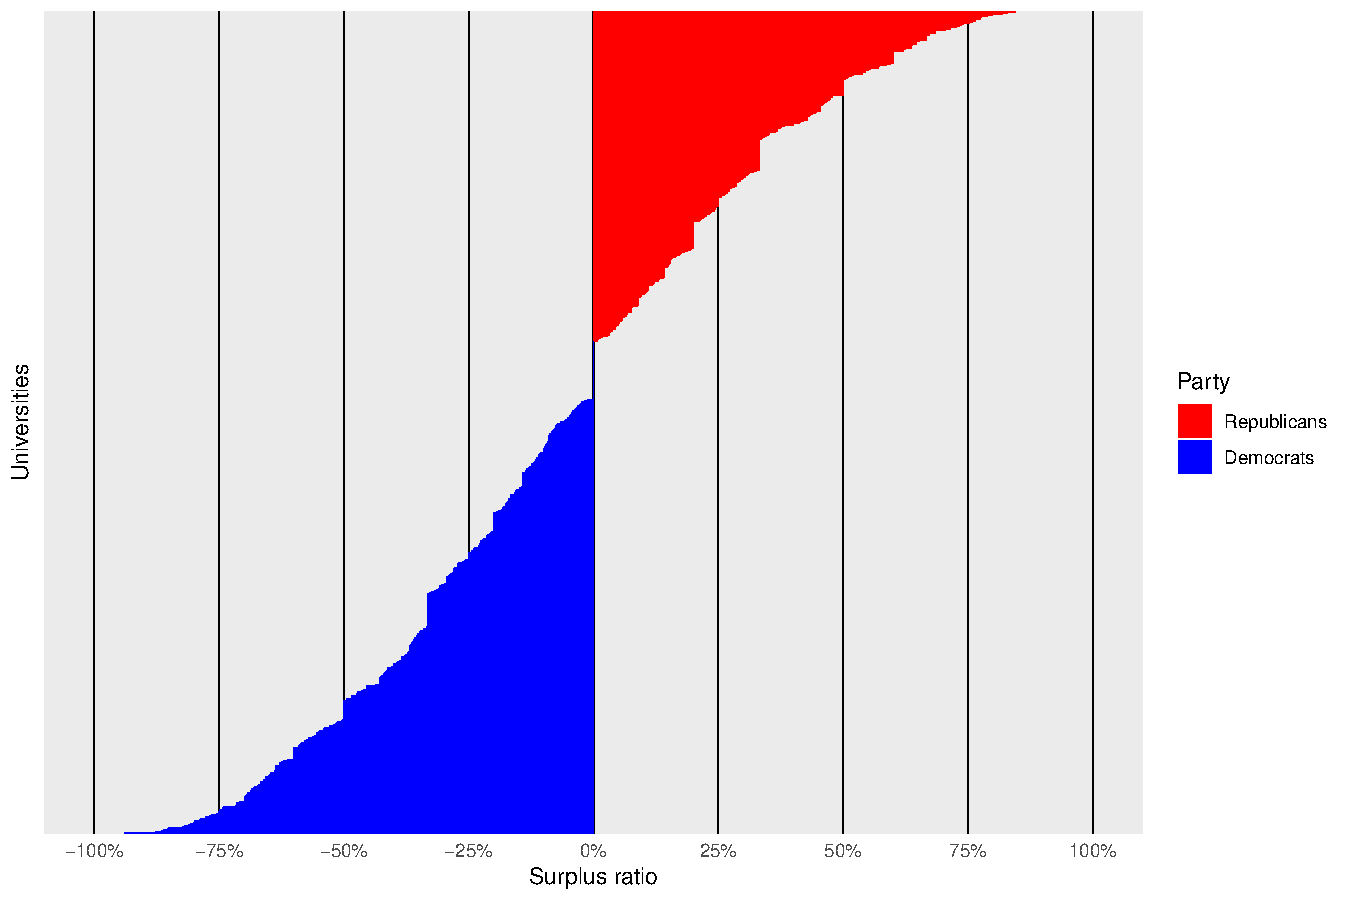
\includegraphics[width=0.95\textwidth]{images/1 surplus_barplot_no_cutoff_full_scale.pdf}
    \caption{Bar plot with all universities and their political surplus ratio.}
    \label{fig:1}
\end{figure}

\begin{figure}[b]
    \centering
    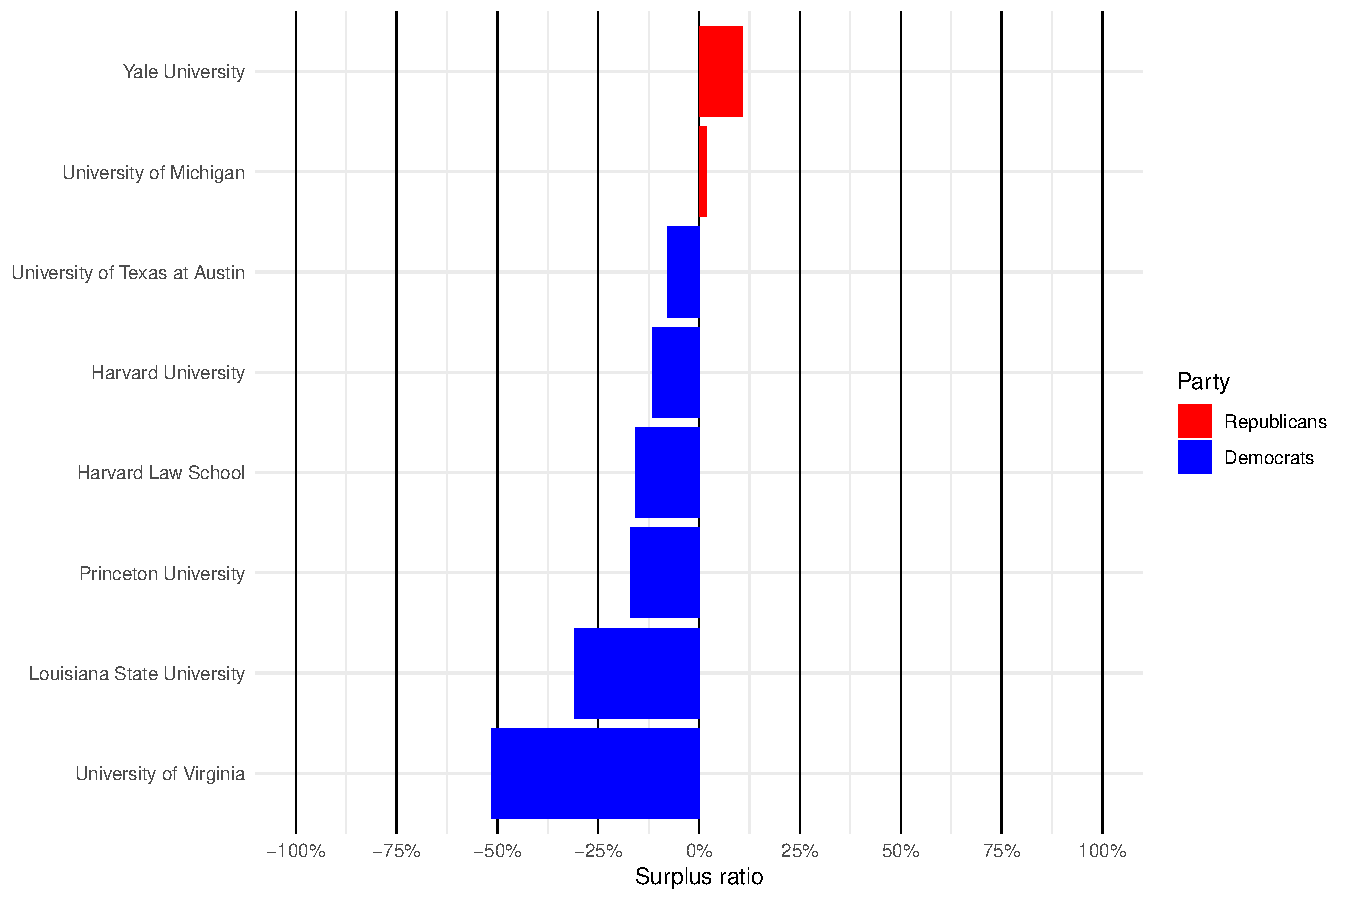
\includegraphics[width=0.95\textwidth]{images/2 surplus_barplot_cutoff=100_full_scale.pdf}
    \caption{Bar plot with the biggest or most politically-focused universities and their political surplus ratio (at least 100 political alumni).}
    \label{fig:2}
\end{figure}

\begin{figure}[b]
    \centering
    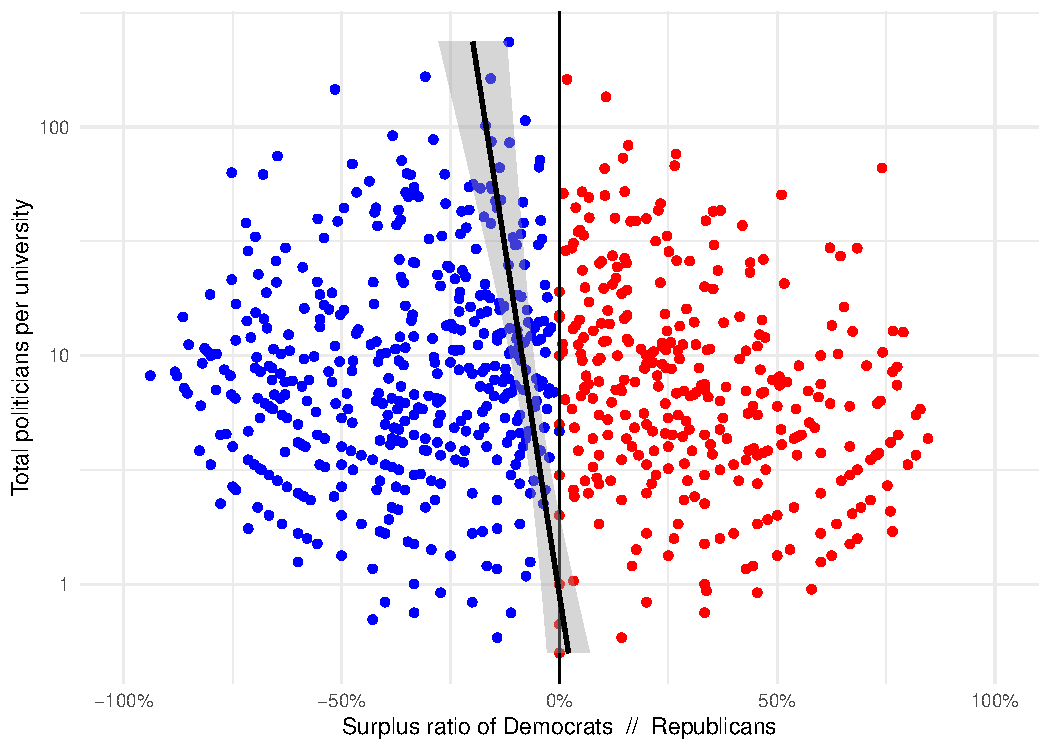
\includegraphics[width=0.95\textwidth]{images/3 surplus_ratio_vs_total_politicians.pdf}
    \caption{Scatter plot with the total number of political alumni per university versus their surplus ratio, including a trendline with a 95\% confidence level.}
    \label{fig:3}
\end{figure}

\begin{figure}[b]
    \centering
    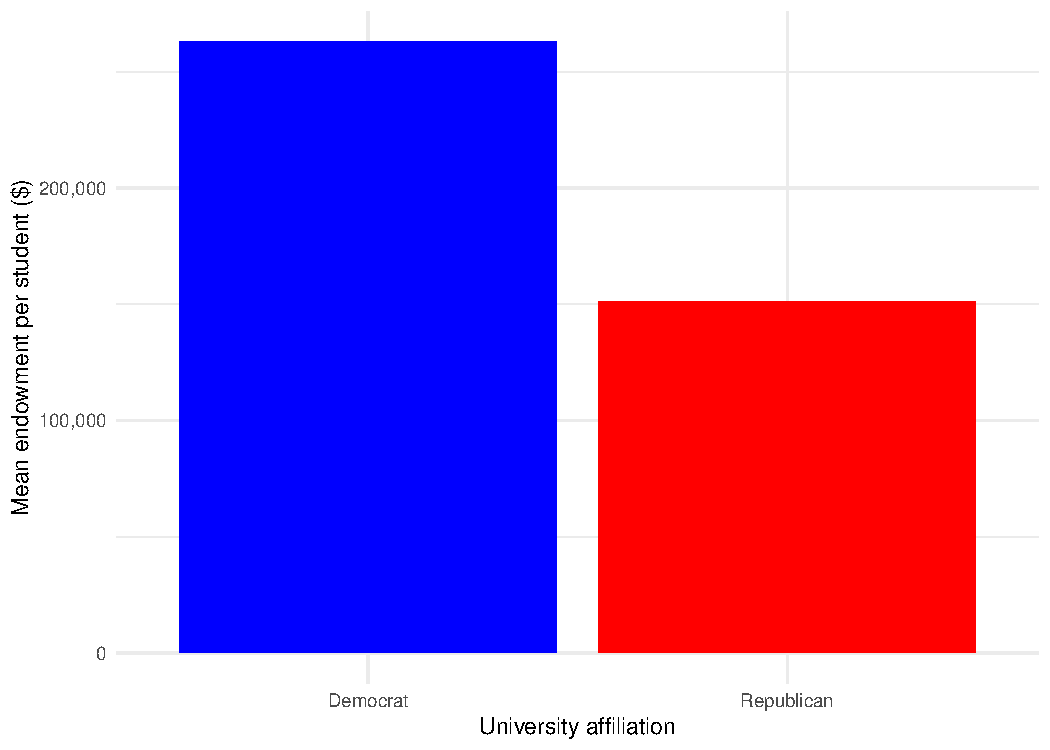
\includegraphics[width=0.95\textwidth]{images/4 endowment_per_university_affiliation_mean.pdf}
    \caption{Bar plot with the mean endowment per student for universities, categorized by the affiliation of the majority of their political alumni.}
    \label{fig:4}
\end{figure}

\begin{figure}[b]
    \centering
    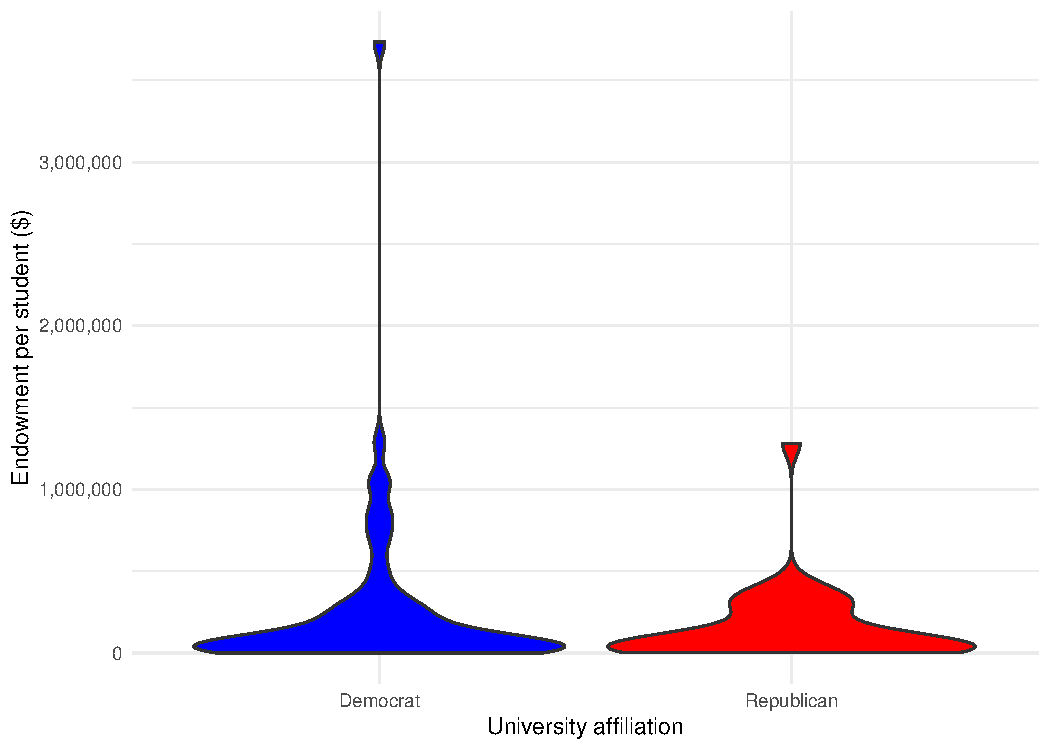
\includegraphics[width=0.95\textwidth]{images/5 endowment_per_university_affiliation_violin_plot.pdf}
    \caption{Violin plot visualizing the distribution of the endowment per student for universities, categorized by the affiliation of the majority of their political alumni.}
    \label{fig:5}
\end{figure}

\begin{figure}[b]
    \centering
    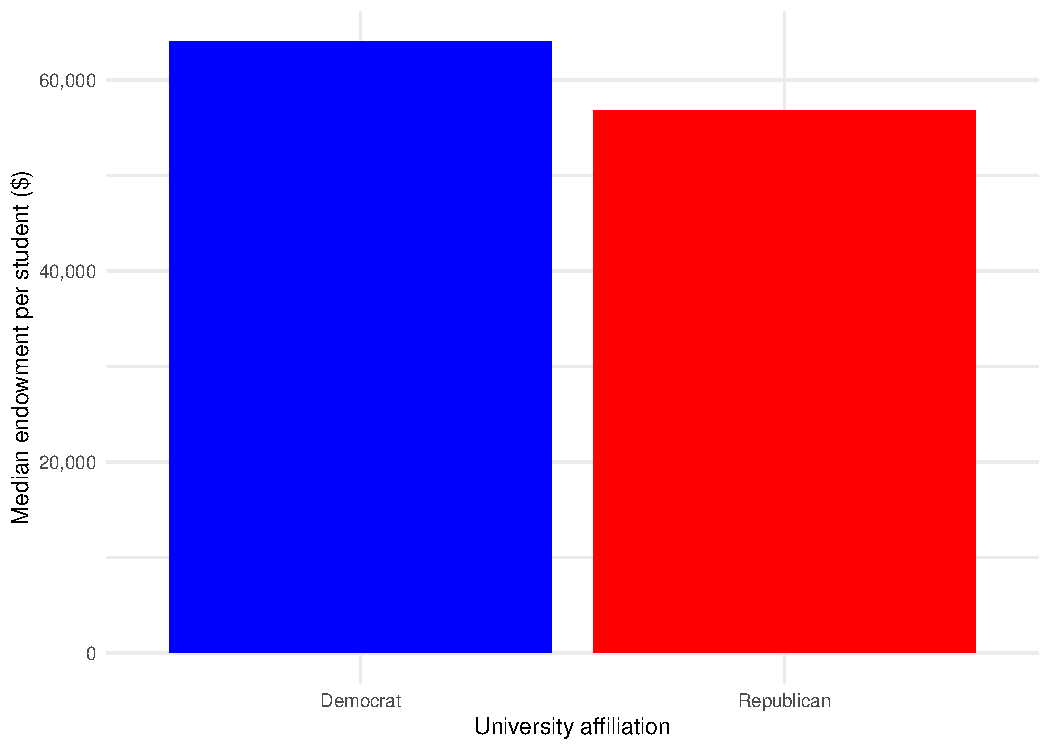
\includegraphics[width=0.95\textwidth]{images/6 endowment_per_university_affiliation_median.pdf}
    \caption{Bar plot with the median endowment per student for universities, categorized by the affiliation of the majority of their political alumni.}
    \label{fig:6}
\end{figure}

\begin{figure}[b]
    \centering
    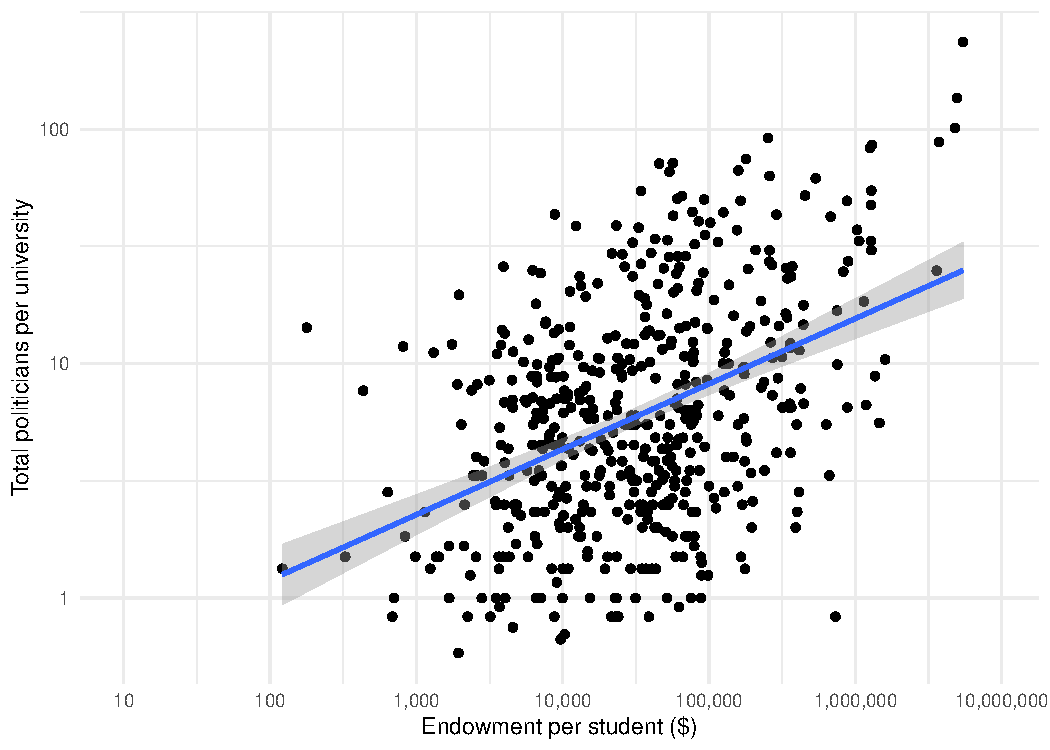
\includegraphics[width=0.95\textwidth]{images/7 endowment_vs_total_politicians.pdf}
    \caption{Scatter plot with the total number of political alumni per university versus their endowment per student, including a trendline with a 95\% confidence level.}
    \label{fig:7}
\end{figure}

In order to explore the relationship between the potential bias of universities and the politicians they produce, we interpret the data visualizations in the following section.

Firstly, the relationship between universities and the political affiliation of their political alumni becomes visible in \autoref{fig:1}. In this figure, there is no filtering applied for the number of alumni, it includes all 1177 universities. A slight general trend can be seen, where universities have more democratic alumni than republican. 

When zooming in, setting the cutoff-value to 100, only the biggest institutions or those that are politically-focused appear, which can be seen in \autoref{fig:2}. The more extreme surplus ratio values are filtered out, which came from very small universities that are very susceptible to changes in numbers, thus unreliable. Important to note is that even without these smaller universities, the trend is still there, even more clearly. 

Increasing this cutoff-value, another observation can be made. This can be noted in \autoref{fig:3}, where the total political alumni per university, so democrats and republicans combined, are plotted against the surplus ratio. A trendline was fitted to this scatterplot, showing the left leaning trend where the more political alumni a university has, the more democratic they are.

For the endowment of universities the mean endowment per student of the universities was plotted, grouped by the political affiliation of the alumni of these universities. This becomes clear in \autoref{fig:4}, where the democratic universities clearly have a larger endowment per student. However, when looking at the violin plot with the same data, seen in \autoref{fig:5}, it can seen that this is partially because of a few wealthy democratic universities, increasing the mean significantly. When looking at the median endowment per student in \autoref{fig:6}, which is less susceptible for these extreme values, we found no significant difference between the different parties.

Disregarding the party of the university, another factor that can play a role is size. This is plotted in \autoref{fig:7}, which contains the total number of political alumni per university against the endowment per student. A trendline was fitted, which shows a general trend that when the number of political alumni per university increases, the more endowment the university has per student. Generally, a 10 fold increase in the number of political alumni results in a 10,000 fold increase in endowment.

\section{Discussion} 

This study set out to examine whether US universities have a bias in the politicians they produce. The data showed that there are certain universities that predominately produce politicians from a specific party, suggesting that perhaps universities do have a political bias. 

An interesting finding was that universities that produce a large amount of politicians also have a larger share of Democrat Party politician alumni.  There are several possible explanations for this result. Perhaps universities that emphasize political engagement are generally more left-leaning. This would lead to more politicians among alumni, with a larger share of them being democrats. An alternative explanation for this finding is that elite colleges might be more left-leaning, producing more democrat politician alumni. Our dataset only contains data from Wikipedia, so these politicians were deemed successful enough to have their own page. Graduating from an elite college could be a signal of 'competence' for voters. Thus, these politicians could be more likely to get elected. Again, these are only speculations about possible causal channels and would need to be properly examined.

Another important finding is that there seems to be relationship between the endowments per student and the number of politician alumni a university produces. The data suggested that universities with high endowments per student also produce more politician alumni. A possible explanation for this pattern is that politicians donate to their alma mater. If some universities already have a surplus of democrats, the donations are skewed towards the Democrat Party. There might be a feedback loop here where colleges are influenced by these donors and educate more politicians in line with their views, thus eventually putting out more Democrat Party politicians. This, again, is pure speculation about what reasons could lie behind these findings.

However, due to a couple limitations these findings should be interpreted with caution. A possible limitation of this study is that within the dataset, there are universities that appear under multiple names. Harvard University appears separately from Harvard Law School, for instance. We chose to treat these institutions as separate entities. However, there is a case to be made for combining these but making the switch is problematic. Creating an algorithm that sorts this is complicated. A solution would be to combine these manually, but because of the high number of entries, this is not feasible.

It is also possible that there are some foreign universities in the dataset because we were not able to filter for specifically the United States. However, this effect seems negligible because we could not find any foreign universities.

For this study, time was not taken into account. A weakness could be that the political stances of alumni of a university might have changed over time. In addition, the age of universities is was not taken into account, so we don't know whether the amount of politicians a university produces might be related to how old it is. A further study with more focus on this variable is suggested.

Additionally, the political leaning is unreliable for small universities. The reason for this is that when the numbers are small, the ratio of democrats and republicans is sensitive. In these cases, even a negligible increase in the number of  alumni associated with one of the parties can drastically change the results. For example, if the a university has 0.25 republican and 11 democratic politician alumni, just one extra republican would drastically alter the results. In \autoref{fig:1}, the most extreme values for both parties are driven by this effect. 

Lastly, the main dataset itself can be seen as problematic, since for instance, not all US politicians are on Wikipedia. Rather, only people that are deemed interesting or successful enough get an entry. Therefore, the dataset is not a fully representative sample for all democrat and republican politicians, which is something to be taken into account. Furthermore, the dataset only contains data up until the year 2018.  This means it excludes the recent political shifts, so the results might be slightly skewed compared to today. 

In spite of these limitations, a conclusion that we can draw from this study is that intricate relationships seem to be present between the variables university, political affiliation and endowment. Our data suggests that within \textit{some} universities, especially the universities that receive higher endowment and have a higher amount of politicians, there seems to be a slight bias towards democratic values. However, this study does not establish causal inference in any of these settings. Researching these questions more rigorously would be necessary to properly answer the issues raised here.

\section{Materials}
\label{sec:materials}
The analysis was carried out entirely in Python and R. The full code can be found on \href{https://github.com/imargit/cracked.egg}{Github}.

\printbibliography
\end{document}

 
